\documentclass[12pt]{article}
\usepackage{enumitem}
\usepackage[T1]{fontenc}
\usepackage[auth-sc,affil-sl]{authblk}
\usepackage{amsmath}
\usepackage{graphicx}
\usepackage{color}
%\usepackage{enumerate}
\usepackage[round]{natbib}
%\usepackage{url} % not crucial - just used below for the URL 
%\usepackage{amsthm}
\usepackage{amssymb}
\usepackage{graphicx}
\usepackage{epstopdf}
\usepackage{hyperref}
\usepackage{alltt}
\usepackage{listings}
\usepackage{array}
\usepackage[noline, boxed, procnumbered, linesnumberedhidden, titlenumbered]{algorithm2e}
\usepackage[firstpage]{draftwatermark}
\usepackage[margin=1in]{geometry}  %%jcgs has own margins

%\pdfminorversion=4
% NOTE: To produce blinded version, replace "0" with "1" below.
\newcommand{\blind}{0}

\newcommand{\secref}[1]{Section~\ref{#1}}
\newcommand{\tblref}[1]{Table~\ref{#1}}
\newcommand{\figref}[1]{Figure~\ref{#1}}
\newcommand{\thmref}[1]{Theorem~\ref{#1}}
\newcommand{\algref}[1]{Algorithm~\ref{#1}}
\newcommand{\funref}[1]{Function~\ref{#1}}
\newcommand{\listingref}[1]{Listing~\ref{#1}}

\newcommand{\eg}{{\em e.g.}}
\newcommand{\ith}{$i^{th}$}
\newcommand{\cut}[1]{}
\newcommand{\todo}[1]{{\bf\em TODO:} #1}

\setlist[enumerate]{itemsep=-1mm}

% DON'T change margins - should be 1 inch all around.
\cut{
\addtolength{\oddsidemargin}{-.5in}%
\addtolength{\evensidemargin}{-.5in}%
\addtolength{\textwidth}{1in}%
\addtolength{\textheight}{1.3in}%
\addtolength{\topmargin}{-.8in}%
}

\begin{document}

\def\spacingset#1{\renewcommand{\baselinestretch}%
{#1}\small\normalsize} \spacingset{1}


%%%%%%%%%%%%%%%%%%%%%%%%%%%%%%%%%%%%%%%%%%%%%%%%%%%%%%%%%%%%%%%%%%%%%%%%%%%%%%

\if0\blind
{
  \title{\bf Accurate and Model-Independent\\
  Partial Dependence Plots}

  \author{Terence Parr and James Wilson\\
      Department of Data Science\\
      University of San Francisco\\
}
  \maketitle
} \fi

\if1\blind
{
  \bigskip
  \bigskip
  \bigskip
  \begin{center}
    {\LARGE\bf Title}
\end{center}
  \medskip
} \fi

\bigskip
\begin{abstract}
Pithy abstract here.
\end{abstract}

\noindent%
{\it Keywords:} 
\vfill

\newpage
%\spacingset{1.5} % DON'T change the spacing!
\section{Introduction}
\label{sec:intro}

In practice, interpreting a machine learning model is just as important as obtaining an accurate model. Feature importance is one such interpretation tool, which indicates the relative predictive power of each feature and is helpful when making business decisions. For example, in a model predicting apartment rent prices, the important features often identify what renters are willing to pay for. On the other hand, feature importance does not identify the relationship itself between features (independent variables) $x_i$ and the target (dependent) variable $y$.  Knowing these relationships tells model users a great deal about their data and, indirectly, the associated real-world population. For example, public health officials might be interested in how years of education affect body weight, given a set of observations sampled from a population.

Given just one or two features, a plot of $x_i$ versus $y$ lets us visualize the exact relationship of each feature and $y$.  Because we cannot visualize more than three dimensions, however, this approach does not work for data sets with more than two features.

To get around this limitation, traditional marginal plots project other axes onto the axis associated with the feature of interest.  That means that marginal plots do not isolate the specific contribution of $x_i$ to $y$. For example, a marginal plot of sex (male/female) versus body weight would likely show that, on average, men are heavier than women. While true, men are also taller than women on average, which likely accounts for most of the difference in average weight. It's unlikely that two ``identical'' people, differing only in sex, would be appreciably different in weight.  

As another example, consider the marginal plot of the number of bathrooms versus price shown in \figref{fig:baths_price}(a) (New York City apartment rent data from Kaggle). One would expect a near-linear relationship for the net effect of the number of bathrooms on price, but the marginal plot implausibly suggests that moving from no bathrooms to one bathroom does not affect the price.   The apartment prices shown in the marginal plot include the effect of all other features for each apartment.

\cite{PDP} introduced partial dependence (PD) plots as a way to extract and visualize the dependence of $y$ on one or two features of interest. \figref{fig:baths_price}(b) shows the (zero-centered) PD of rent price on the number of bathrooms as a black line. The partial dependence line is the average of the blue lines, which represent the individual conditional expectation (ICE) plots of \cite{ICE}.  In this case, the ICE lines depict the model prediction contributions for a single observation as the bathroom feature shifts through all possible number of bathrooms. Because PD plots represent an average across observations, they can hide a great deal of variability, so it is helpful to combine PD and ICE plots.

The partial dependence plot seems to follow the marginal plot except for the three and four bathroom apartments, where it levels off. This is counterintuitive and exposes an issue with PD plots. While PD plots are model-agnostic, they are not model-independent and are subject to the strengths and weaknesses of the model used to make predictions. In \figref{fig:baths_price}(b), the model is a Random Forest(tm) (RF) and RFs cannot extrapolate beyond their support range.  The data set has few apartments with three and four bathrooms, as shown by the lack of blue dots in that range of the marginal plot, so the price predictions appear to flatten out after two bathrooms.  \figref{fig:baths_price}(c) shows the PD/ICE plot for the exact same data set but using a linear model (with Lasso regularization).
 
a result of collinearity with, for example, the number of bedrooms.
 
as long as these features are not strongly collinear with the remaining features. The interaction between variables causes marginal plots


define what we are actually looking for: controlling for other variables or net effect. All other features being equal. partial derivative.



 \begin{figure}[htbp]
\begin{center}
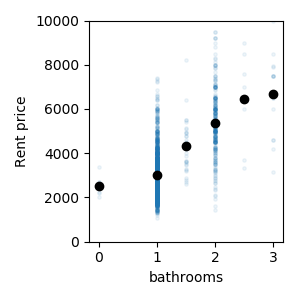
\includegraphics[scale=0.7]{images/baths_vs_price.png}
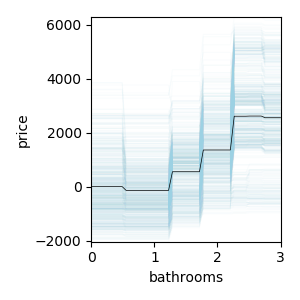
\includegraphics[scale=0.7]{images/baths_vs_price_pdp.png}
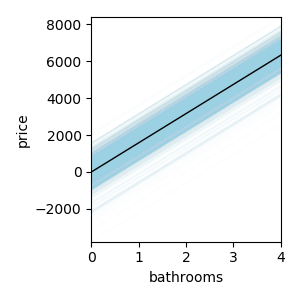
\includegraphics[scale=0.7]{images/baths_vs_price_pdp_lm.png}
\caption{{\bf  Marginal plot and PDP/ICE plot of bathrooms versus rent price}}
\label{fig:baths_price}
\end{center}
\end{figure}

After controlling for all other features,




\section{Related work}

PDP math shows that features added or multiplied times the remaining F approximation completely describe the partial dependence; I assume that means that interactions are not a problem.

do we need to talk about LIME?
 
This python package seems to do PDP, LIME etc... https://github.com/oracle/Skater

\section{Future work}

This work describes regressors only, ignoring partial dependence for classifiers.  Research reveals no papers or implementation for classifiers. Friedman, however, briefly describes a partial dependence mechanism for classification whereby $k$-class logistic regression (one-versus-rest) equations indicate the probability of seeing class $k$ at $\bf{x}$.  This suffers from the same interaction-based bias as the regressor model.

Actually, the R version of personal dependence may actually do this. See https://christophm.github.io/interpretable-ml-book/pdp.html where he describes PDP for cancer prediction and gets probabilities out.

\section{Conclusion}
\label{sec:conc}

\bibliographystyle{apalike}

\bibliography{mipd}
\end{document}